\chapter{Research Design \& Application}
\label{ch:design}
As discussed in the literature review this research has a focus on the negotiation of the agents. Using different methods and techniques an attempt is made to optimize a production process. We search for an approximate-optimal solution while the optimal solution is unknown. Based on learning methods from decentralized holonistic methods, utility and negotation domains a simulation can be build which can be applied to the production process. 

The system where the  decentralized solution will be applied is a de-mineralized water plant as described in the introduction and problem chapters (\cref{ch:intro}).

As explained in the literature, a negotiation problem can be characterized by a negotiation domain (who negotiates and what to negotiate about), an interaction protocol (which rules govern the negotiation process) and a set of decision mechanisms or strategies that guide the negotiating agents through every phase of the interaction protocol \cite{fatima2014principles}.

For the scope of this work, we assume a multi-attribute negotiation domain, where a deal or solution to the problem is defined as the set of attributes (issues), and each one of them can be in a certain range.

The coding will be done in Java from scratch. Multiple open-source systems area available, including Jadex, which is perfect for communication research in a Multi-Agent System~\cite{kravari2015survey}. However since most of these systems are very comprehensive little adjustments which are necessary for our research are not conceivable.

%\section{Mapping of Literature on usecase}
%	\begin{tabular}{p{2cm}|p{2cm}|p{2cm} l l |p{3cm}}
%		& Category & Literature & & & Usecase\\
%		\hline \hline
%		Real-time & Physical (process) & Object/service oriented programming & & & Operations:
%		\begin{itemize} 	
%			\item Production Guarantee (leveringszekerheid) 
%			\item Batch Production 
%			\item Ions, flow, Ammonia (water softening)		
%		\end{itemize}\\
%		\hline
%		Real-time & Sensing & Programmable Logic Controller; Real-time Monitor & \multirow{2}{*}{\rotatebox[origin=c]{90}{Holonic, Cyber-Physical}} & %\multirow{3}{*}{\rotatebox[origin=c]{90}{e-manufacturing}}
%		& Sensors (mineral, temperature, softening, ammonia, flow)\\
%		\hline
%		Sec - Min & Analysis & Agent; BDI; Data Analysis; Machine Learning & & & Predictive/Condition based Maintenance\\
%		\hline
%		Hours - Weeks & Work order/Action & Planning; MAS; Scheduling; Game Theory & \multirow{2}{*}{\rotatebox{90}{Negotiation}}& & Work flow; Logisics Spare Parts; Process control feedback; integrated supply chain
%		
%	\end{tabular}
%	

%\section{Mapping of Negotiation}


\section{Demineralization of water}
As discussed in the introduction, the usecase where an Multi-Agent system for production will be implemented is a water demineralization plant. An application of this new model will be applied to a large plants that creates de-mineralized water. By removing all the ions from common water, de-mineralized water is obtained. This water is used for many processes, and has many applications. In this plant specifically it is used for the steam turbines, which generate electricity. By burning the by-product, heat is generated, which creates steam to power the turbines. 

\begin{figure}
	\centering
	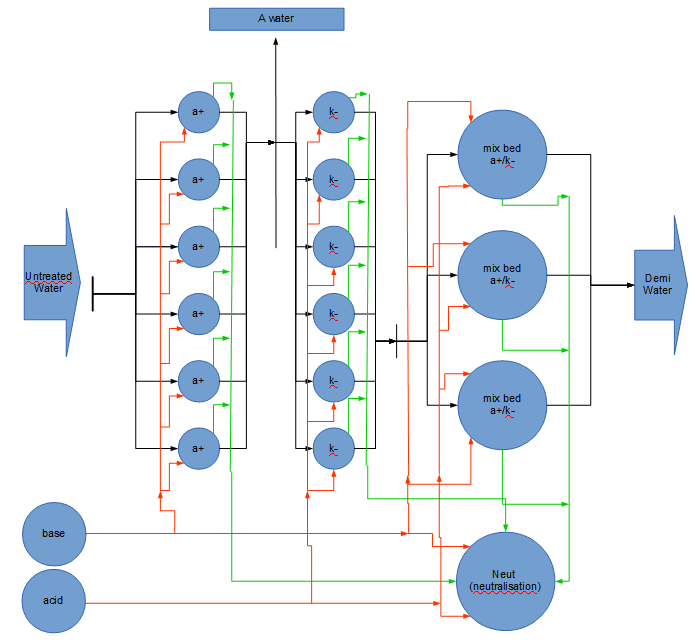
\includegraphics[width=1\linewidth]{img/demi-plant}
	\caption{An overview of a water demineralization plant.}
	\label{fig:demi-plant}
\end{figure}

Minerals are removed from water by multiple production steps. Most common, and as is implemented in the plant described, is to first remove the positively charged minerals in so called anions. After this the negative charged ions are removed with in a cation filter. To ensure all ions are removed, a final combined ``mixbed'' is used. Here a combination of an anion and cation filter removes the residues.

These filters have to be cleaned every few hours to ensure proper demineralization occurs. For cleaning acid and base are used. By filtering the anion with base the ions that have been retrieved in the filtering are flushed. The residue, still of a base composition, is stored in a storage tank where the combination of the base and acids from the filters is neutralized. This storage tank is called the ''Neut`` as short.

So overall we have 4 kinds of filters, the anions, the cations, the mixbed and the Neut. Each of these filters sorts have multiple of each other, but for simplification we only look at the allocation of resources for these four ''agents``. Within each agent the BDI module will ensure the right task location. This will not be done with negotiation but with the BDI which is retrieved from the experts knowledge.


This structure is that of a holon as can be seen in figure~\ref{fig:holonexample}. As shown in the literature it is based on PROSA by \citet{van1998reference}.
\begin{figure}
	\centering
	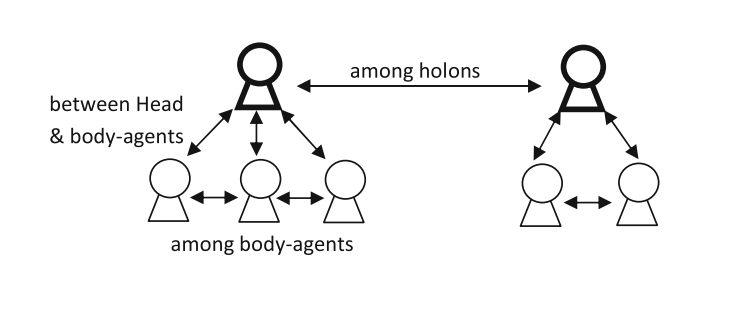
\includegraphics[width=0.7\linewidth]{img/holon_example}
	\caption{An example of the different negotiation between holons from \citet{beheshti2016negotiations}.}
	\label{fig:holonexample}
\end{figure}

\section{Negotiation model}
These 4 rational agents, $M = \{1,2,3, 4\}$, partition 3 issues $N=\{1,2,3\}$: the water that has to be delivered at the end of the process, and the base and acid for cleaning.  This can be simplified to a buyer seller negotiation.

Anion wants to buy as much base as possible, while the minimum amount of water. For the cation, as much acid as possible is required, while still as little water as possible should be produced. The mixbed requires as much as possible acid and base for cleaning. Since it the final production step, it requires the water to be delivered, forcing it to obtain as much water as possible from the cation. Finally there is the Neut which wants as little base and acid as possible. Also the base and acid should be levelled out as much as possible to attempt to stay as close to a pH of $7$. 

The above abstractly is translated to an unit interval $[0, 1]$ in $\mathbb{R}$. Since we have $3$ issues, the unit hypercube $[0, 1]^3$ in  $\mathbb{R}^3$. This results in a possible negotiation domain $\Omega = [0,1]$

The utility function for each agent $u_i(x)$ is convex, and normalized between $[0, 1]^3$. Each agent has a reservation utility $ru_i$. Any offer below this reservation utility is unacceptrable. This means that the set of feasible offers is $A = \{ x\in [0,1]^3|u_i\(x)\geq ru_i}$. Since the function is convex, $A$ is also.  

The protocol is based on the method as proposed by \citet{wu2009efficient}. Here an multilateral multi-issue method for negotiation about the allocation of resources is given. 

Since the agents have no knowledge regarding the states of the other agents. Furthermore, each agent will have its own utility function which is private. 

The negotiation takes place in rounds $n\in \mathbb{N} $. $\mathbf{x}_i \in (0,1)^2$ denotes a bid of agent $i \in N$ in a round and $x_{i,j}\in \mathbf{x}_i$  denote the amount of issue $j \in M$.

%Using BDI in each agent, the anion will know which filter to use when, and when to clean them. This intelligence can be learned. There is a limit on the amount of water, base or acid.

%Head tries to increase the holon utility as a whole, and this does not contradict the increase in body-agent utility. In other words, Head wants to increase holon’s utility, and is willing to do this according to body-agent preference. 

\begin{figure}
	\centering
	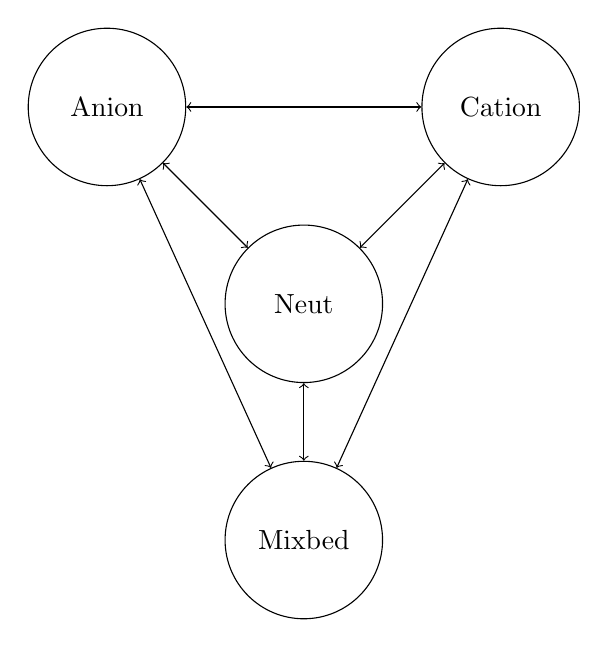
\begin{tikzpicture}
	\node[circle,draw, minimum size=2cm] (A) at  (0,0) {Neut};
	\node[circle,draw, minimum size=2cm] (B) at (-2.5,2.5) {Anion};
	\node[circle,draw, minimum size=2cm] (C) at (2.5,2.5) {Cation};
	\node[circle,draw, minimum size=2cm] (D) at (0,-3) {Mixbed};
	
	\draw[<->] (A) -- (B);
	\draw[<->] (A) -- (C);
	\draw[<->] (A) -- (D);
	\draw[<->] (B) -- (C);
	\draw[<->] (B) -- (D);
	\draw[<->] (C) -- (D);
	\end{tikzpicture}
	\caption{A simplified representation.}
	\label{fig:agent-plant}
\end{figure}


\begin{figure}
	\centering
	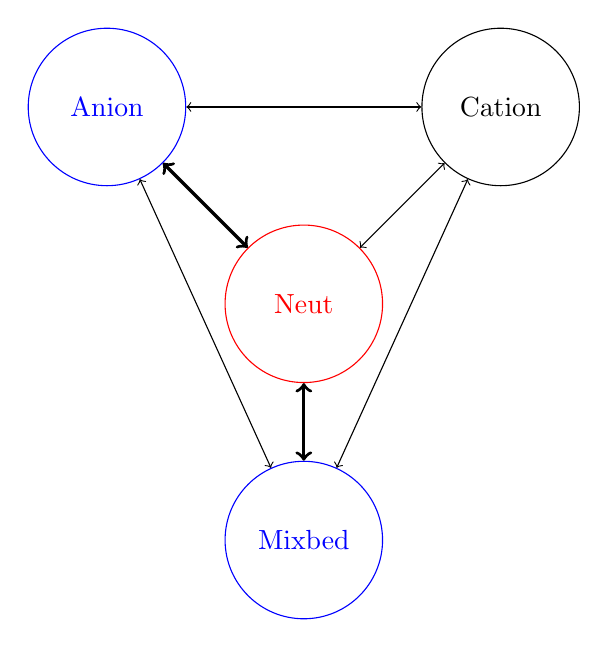
\begin{tikzpicture}
	\node[circle,draw, red, minimum size=2cm] (A) at  (0,0) {Neut};
	\node[circle,draw, blue, minimum size=2cm] (B) at (-2.5,2.5) {Anion};
	\node[circle,draw, minimum size=2cm] (C) at (2.5,2.5) {Cation};
	\node[circle,draw, blue, minimum size=2cm] (D) at (0,-3) {Mixbed};
	
	\draw[very thick, <->] (A) -- (B);
	\draw[<->] (A) -- (C);
	\draw[very thick, <->] (A) -- (D);
	\draw[<->] (B) -- (C);
	\draw[<->] (B) -- (D);
	\draw[<->] (C) -- (D);
	\end{tikzpicture}
	\caption{Base negotiation. Red indicates seller, blue buyer}
	\label{fig:agent-plant-base}
\end{figure}

\begin{figure}
	\centering
	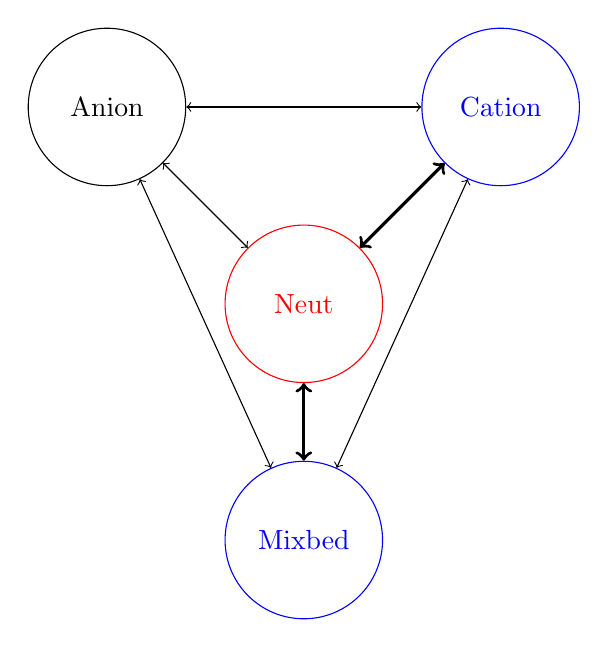
\begin{tikzpicture}
	\node[circle,draw, red, minimum size=2cm] (A) at  (0,0) {Neut};
	\node[circle,draw, minimum size=2cm] (B) at (-2.5,2.5) {Anion};
	\node[circle,draw, blue, minimum size=2cm] (C) at (2.5,2.5) {Cation};
	\node[circle,draw, blue, minimum size=2cm] (D) at (0,-3) {Mixbed};
	
	\draw[<->] (A) -- (B);
	\draw[very thick, <->] (A) -- (C);
	\draw[very thick, <->] (A) -- (D);
	\draw[<->] (B) -- (C);
	\draw[<->] (B) -- (D);
	\draw[<->] (C) -- (D);
	\end{tikzpicture}
	\caption{Acid negotiation}
	\label{fig:agent-plant-acid}
\end{figure}

\begin{figure}
	\centering
	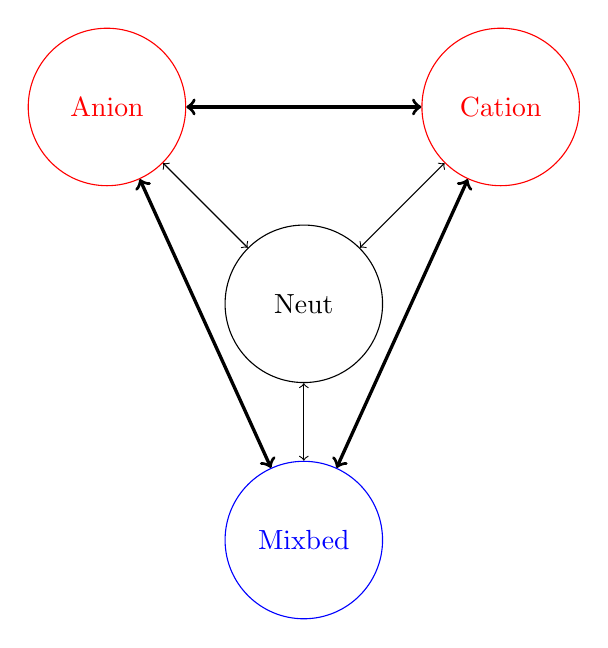
\begin{tikzpicture}
	\node[circle,draw,  minimum size=2cm] (A) at  (0,0) {Neut};
	\node[circle,draw, red, minimum size=2cm] (B) at (-2.5,2.5) {Anion};
	\node[circle,draw, red, minimum size=2cm] (C) at (2.5,2.5) {Cation};
	\node[circle,draw, blue, minimum size=2cm] (D) at (0,-3) {Mixbed};
	
	\draw[<->] (A) -- (B);
	\draw[<->] (A) -- (C);
	\draw[<->] (A) -- (D);
	\draw[very thick, <->] (B) -- (C);
	\draw[very thick, <->] (B) -- (D);
	\draw[very thick, <->] (C) -- (D);
	\end{tikzpicture}
	\caption{Water negotiation}
	\label{fig:agent-plant-water}
\end{figure}


\section{Details of the Agents}
Each agent has its own characteristics on which the system will run. The basis consists of the different sub agents. The head agent will know the state of the sub agents and will negotation on heave of the entire group. 

Important to note is that the utility function is required to be convex. 
\subsection{Anion}
The anion is the first filter where the untreated water will arrive. The filters have different charatistics and it is the job of the head to decide on the filters task. SOme will be pauzed, some will filter, and others will be cleaned. 
\subsubsection{Utility function}
As described in \citet{wong2010multi}, it is possible by combining the input into the utiltiy function of the agent. This is shown in \cref{fig:wongutiltiyneuralnetwork}. 

At first a simple linear utiltiy function will be used: the less water, the higher the utility. Also, the more base, the higher the utility. This has a limit, depending on the reservation function as shown in \cref{fig:anionreservationfunction}.


\begin{figure}
	\centering
	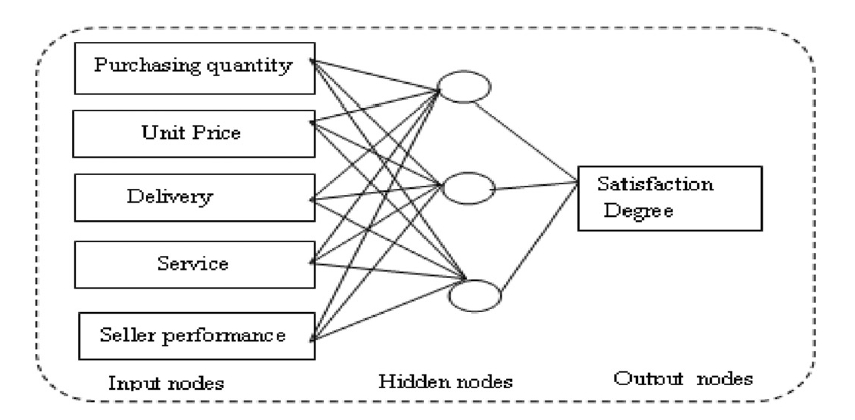
\includegraphics[width=0.7\linewidth]{img/wong_utiltiy_NeuralNetwork}
	\caption{An example where the utility function is modelled with a Neural Network. \citep{wong2010multi}.}
	\label{fig:wongutiltiyneuralnetwork}
\end{figure}

\begin{figure}
\centering
	\begin{tikzpicture}[domain=0.15:4]
	%\draw[very thin,color=gray] (0.01,0.01) grid (3.9,3.9);
	\draw[->] (0.02,0) -- (4.2,0) node[below] {$Water$};
	\draw[->] (0,0.02) -- (0,4.2) node[left] {$Base$};% node[pos=0.25, left] {$200 m^3 / hr$};
	\draw[color=black] plot (\x,{0.07*exp(\x)}) node[left] {$R_A$};
	\end{tikzpicture}
	\label{fig:anionreservationfunction}
	\caption{The reservation function for the Anion filter: the more water is filtered and given, the more base it requires.}
\end{figure}

A very important input to the utility function is that of the belief in the other agents. These will not be formally modelled, as in Kripke worlds e.g., but can still be used as input to the utility function. 
%\begin{figure}
%	\centering
%	\begin{tikzpicture}
%[domain=0.15:4]
%%\draw[very thin,color=gray] (0.01,0.01) grid (3.9,3.9);
%\draw[->] (0.02,0) -- (4.2,0) node[below] {$Water$};
%\draw[->] (0,0.02) -- (0,4.2) node[left] {$Base$}; %node[pos=0.25, left]   {$200 m^3 / hr$} 
%\draw[scale=0.5,domain=0.1:7.872,smooth,variable=\x,red] plot({\x},{(1/ (\x-8))+8 } );
%
%\end{tikzpicture}
%\label{fig:rcurveofanion}
%\caption{An illustrative sketch reservation curve of the offer space for the anion}
%\end{figure}

\subsubsection{Facts}
The following facts and rules are part of the Anion.

\begin{enumerate}
	\item
	Knowledge of anion head about the sub-agents:
	\begin{itemize}
		\item {$\{A_1, ..., A_6\}$ can process $a$ amount of water}
		\item {$\{A_1, ..., A_6\}$ needs to be cleaned after $b$ water}
		\item {$\{A_1, ..., A_6\}$ has filtered $c$ amount of water}
		\item {$\{A_1, ..., A_6\}$ needs $d$ base to clean}
		\item {$\{A_1, ..., A_6\}$ needs $e$ time to clean}
	\end{itemize}
	\item
	Currently $x$ amount of water being filtered 
	\item
	Currently $Z \subseteq \{A_1, ..., A_6\}$ filter being used for water filtering
	\item
	Currently $Y \subseteq \{A_1, ..., A_6\}$ filter being used for cleaning
	\item
	Currently $w$ amount of base being used for cleaning
\end{enumerate}

\begin{figure}[h]
	
	\centering
	\begin{tikzpicture}
	
	\node[circle,draw,  minimum size=1cm] (A1) at  (0,0) {A$_1$};
	\node[circle,draw,  minimum size=1cm] (A2) at  (0,-1.5) {A$_2$};
	\node[circle,draw,  minimum size=1cm] (A3) at  (0,-3) {A$_3$};
	\node[circle,draw,  minimum size=1cm] (A4) at  (0,-4.5) {A$_4$};
	\node[circle,draw,  minimum size=1cm] (A5) at  (0,-6) {A$_5$};
	\node[circle,draw,  minimum size=1cm] (A6) at  (0,-7.5) {A$_6$};
	%\draw  (0,-2.5) ellipse (1 and 3.4);
	
	\node[ellipse,  draw, minimum height =9cm, minimum width = 2.5cm ] (A) at (0,-3.75) {Anion};
	
	\end{tikzpicture}
	\caption{Anion head and sub-agents}
	\label{fig:anion-head-sub}
	
\end{figure}

\clearpage
\subsection{Cation}
The cation is the second aspect of the water cleaning process and where the positively charged ions are removed. It cleans itself with acid. A overview of the filter is shown in \cref{fig:cation-head-sub}.

The utility is very similar to that of the Anion but a preference over acid instead of base is required. The reservation function is shown in \cref{fig:cationreservationfunction}.
\begin{figure}
	\centering
	\begin{tikzpicture}[domain=0.15:4]
	%\draw[very thin,color=gray] (0.01,0.01) grid (3.9,3.9);
	\draw[->] (0.02,0) -- (4.2,0) node[below] {$Water$};
	\draw[->] (0,0.02) -- (0,4.2) node[left] {$Acid$};% node[pos=0.25, left] {$200 m^3 / hr$};
	\draw[color=black] plot (\x,{0.07*exp(\x)}) node[left] {$R_C$};
	\end{tikzpicture}
	\label{fig:cationreservationfunction}
	\caption{The reservation function for the Cation filter: the more water is filtered and given, the more acid it requires.}
\end{figure}




\begin{figure}[h]
	\centering
	\begin{tikzpicture}
	
	\node[circle,draw,  minimum size=1cm] (C1) at  (0,0) {C$_1$};
	\node[circle,draw,  minimum size=1cm] (C2) at  (0,-1.5) {C$_2$};
	\node[circle,draw,  minimum size=1cm] (C3) at  (0,-3) {C$_3$};
	\node[circle,draw,  minimum size=1cm] (C4) at  (0,-4.5) {C$_4$};
	\node[circle,draw,  minimum size=1cm] (C5) at  (0,-6) {C$_5$};
	\node[circle,draw,  minimum size=1cm] (C6) at  (0,-7.5) {C$_6$};
	%\draw  (0,-2.5) ellipse (1 and 3.4);
	
	\node[ellipse,  draw, minimum height =9cm, minimum width = 2.5cm ] (C) at (0,-3.75) {Cation};
	
	\end{tikzpicture}
	\caption{Cation head and sub-agents}
	\label{fig:cation-head-sub}
\end{figure}
\subsubsection{Facts}
The following facts and rules are part of the Anion.

\begin{enumerate}
	\item
	Knowledge of cation head about the sub-agents:
	\begin{itemize}
		\item {$\{C_1, ..., C_6\}$ can process $a$ amount of water}
		\item {$\{C_1, ..., C_6\}$ needs to be cleaned after $b$ water}
		\item {$\{C_1, ..., C_6\}$ has filtered $c$ amount of water}
		\item {$\{C_1, ..., C_6\}$ needs $d$ acid to clean}
		\item {$\{C_1, ..., C_6\}$ needs $e$ time to clean}
	\end{itemize}
	\item
	Currently $x$ amount of water being filtered 
	\item
	Currently $Z \subseteq \{C_1, ..., C_6\}$ filter being used for water filtering
	\item
	Currently $Y \subseteq \{C_1, ..., C_6\}$ filter being used for cleaning
	\item
	Currently $w$ amount of acid being used for cleaning
\end{enumerate}

\clearpage
\subsection{Mixbed}
The mixbed is where the final cleaning occurs (see \cref{fig:mixbed-head-sub}). It is also the agent responsible for the end water delivery. Since it consists of a mixture off anion and base it has three issues it desires. These are shown in \cref{fig:mixreservationfunction1, fig:mixreservationfunction2}.


\begin{figure}[h]
	\centering
	\begin{tikzpicture}
	
	\node[circle,draw,  minimum size=1cm] (M1) at  (0,0) {M$_1$};
	\node[circle,draw,  minimum size=1cm] (M2) at  (0,-1.5) {M$_2$};
	\node[circle,draw,  minimum size=1cm] (M3) at  (0,-3) {M$_3$};
	%\draw  (0,-2.5) ellipse (1 and 3.4);
	
	\node[ellipse,  draw, align=left, minimum height =5cm, minimum width = 2cm ] (A) at (0,-1.5) { \rotatebox{90}{\parbox{1cm}{Mixbed \\\\ \\ \\}}};
	
	\end{tikzpicture}
	\caption{Mixbed head and sub-agents}
	\label{fig:mixbed-head-sub}
\end{figure}


\begin{figure}
	\centering
	\begin{tikzpicture}[domain=1.3:4]
	%\draw[very thin,color=gray] (0.01,0.01) grid (3.9,3.9);
	\draw[->] (0.02,0) -- (4.2,0) node[below] {$Water$};
	\draw[->] (0,0.02) -- (0,4.2) node[left] {$Acid$};% node[pos=0.25, left] {$200 m^3 / hr$};
	\draw[color=black] plot (\x,{(1/(\x-1))+1}) node[above] {$M_C$};
	\end{tikzpicture}
	\label{fig:mixreservationfunction1}
	\caption{The reservation function for the Mixbed filter: a bear minimum of water is required at all times, and thus a bare minimum of cleaning acid.}
\end{figure}

%
%
\begin{figure}
	\centering
	\begin{tikzpicture}[domain=1.3:4]
	%\draw[very thin,color=gray] (0.01,0.01) grid (3.9,3.9);
	\draw[->] (0.02,0) -- (4.2,0) node[below] {$Water$};
	\draw[->] (0,0.02) -- (0,4.2) node[left] {$Base$};% node[pos=0.25, left] {$200 m^3 / hr$};
	\draw[color=black] plot (\x,{(1/(\x-1))+1}) node[above] {$M_C$};
		\end{tikzpicture}
		\label{fig:mixreservationfunction2}
		\caption{The reservation function for the Mixbed filter: a bear minimum of water is required at all times, and thus a bare minimum of cleaning base.}
	\end{figure}
\subsubsection{Facts}
The following facts and rules are part of the Mixbed.

\begin{enumerate}
	\item
	Knowledge of anion head about the sub-agents:
	\begin{itemize}
		\item {$\{M_1, M_2, M_3\}$ can process $a$ amount of water}
		\item {$\{M_1, M_2, M_3\}$ needs to be cleaned after $b$ water}
		\item {$\{M_1, M_2, M_3\}$ has filtered $c$ amount of water}
		\item {$\{M_1, M_2, M_3\}$ needs $d$ base to clean}
		\item {$\{M_1, M_2, M_3\}$ needs $e$ time to clean}
		\item {$\{M_1, M_2, M_3\}$ needs $f$ acid to clean}
	\end{itemize}
	\item
	Currently $x$ amount of water being filtered 
	\item
	Currently $Z \subseteq \{M_1, M_2, M_3\}$ filter being used for water filtering
	\item
	Currently $Y \subseteq \{M_1, M_2, M_3\}$ filter being used for cleaning
	\item
	Currently $w$ amount of base being used for cleaning
	\item
	Currently $v$ amount of acid being used for cleaning
\end{enumerate}

\clearpage
\subsection{Neut}
The neut is the agent responisble for the division of the amount of Acid and base. Since it wants to stay as pH neutral as possible, it requires an even distribution of base and acid between the agents. This is shown in \cref{fig:neutreservationcurve}.
\begin{figure}
	\centering
      \begin{tikzpicture}
      
      [domain = 0.1:3.9]
      
      \draw[->] (0.02,0) -- (4.2,0) node[right] {$Base$}; 
      \draw[->] (0,0.02) -- (0,4.2) node[left] {$Acid$};
      \draw[scale=0.5,domain=0:6,smooth,variable=\x,blue] plot ({\x},{\x+2}) node[left] {$R_{N1}$};
      
      \draw[scale=0.5,domain=2:8,smooth,variable=\x,blue] plot ({\x},{\x-2}) node[right] {$R_{N2}$} ;
      
      \end{tikzpicture}
		\caption{The neut reservation curve. A near equal division is required.}
		\label{fig:neutreservationcurve}
\end{figure}
\subsubsection{Facts}
The following facts and rules are part of the Neut.

\begin{enumerate}
	\item
	Current $a$ amount of acid being used.
	\item
	Current $b$ amount of base being used.
	
\end{enumerate}


%\begin{figure}
%	\centering
%\begin{tikzpicture}
%[domain=0.15:4]
%%\draw[very thin,color=gray] (0.01,0.01) grid (3.9,3.9);
%\draw[->] (0.02,0) -- (4.2,0) node[below] {$Water$};
%\draw[->] (0,0.02) -- (0,4.2) node[left] {$Acid$}; %node[pos=0.25, left]   {$200 m^3 / hr$} 
%\draw[scale=0.5,domain=0.1:7.872,smooth,variable=\x,blue] plot({\x},{(1/ (\x-8))+8 } );
%
%\end{tikzpicture}
%\label{fig:rcurveofcation}
%\caption{An illustrative sketch reservation curve of the offer space for the cation}
%\end{figure}


\section{Evaluation}
Data from a true demi plant is used to see wether the solution will be optimized.

\clearpage
\section{Algorithm}

\begin{algorithm}
	\KwData{Each agent’s utility function $u_i(x)$, reservation utility $ru_i$, and concession strategy $s_i(t)= 1,2,...,T$}
	\KwResult{Negotiation Agreement}
	initialization: Each agent proposes a preferred offer $xî_0$\;
	$t\leftarrow1$\;
	Set convergence tolerance: $\delta$\;
	\While{$t\leq T$ and Isconverge == False}
	{
		Determine the agent to propose: i = mod(t,m)\;
		\ForEach{$j\in {1,2,...,m}$}
		{
			\eIf{j == 1}
			{
				Agent $i$ concedes by determining $s_i(t)$\;
				Agent $i$ calculates: $w_{t-1}\leftarrow \frac{1}{m}\sum_{j=1}^{m}x^j_{t-1}$\;
				Agent $i$ proposes $P_{A^i_t}[w_{t-1}]$\;
			}{
				$x^j_i \leftarrow x^j_{t-1}$\;
			}
		}
		\eIf{$\max_{ j \in {1,2,...,m}} \parallel x^j_t-w_{t-1} \parallel < \delta$ }
		{
			IsConverge $\leftarrow $ True\;
		}{
			$t \leftarrow t+1$\;
		}
	}
\caption{Basic algorithm structure from \citet{zheng2015automated}.}
\end{algorithm}

\todos
